\documentclass{standalone}
\usepackage{tikz}
\begin{document}
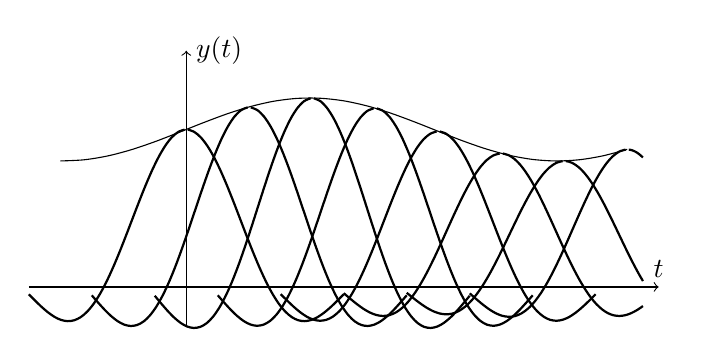
\begin{tikzpicture}[scale=2]
    \draw[->](0,-0.25)--(0,1.5)node[right]{$y(t)$};
    \draw[->](-1,0)--(3,0)node[above]{$t$};


    \draw[]plot[smooth, domain=-0.8:2.8](\x,{1+0.2*sin(2*\x r)});

    \draw[-, thick]plot[smooth,domain=-1:-0.01](\x,{sin(6*(\x) r)/(6*(\x))});
    \draw[-, thick]plot[smooth,domain=0.01:1](\x,{sin(6*(\x) r)/(6*(\x))});

    \draw[-, thick]plot[smooth,domain=-0.6:0.39](\x,{1.141*sin(6*(\x-0.4) r)/(6*(\x-0.4))});
    \draw[-, thick]plot[smooth,domain=0.41:1.4](\x,{1.141*sin(6*(\x-0.4) r)/(6*(\x-0.4))});

    \draw[-, thick]plot[smooth,domain=-0.2:0.79](\x,{1.199*sin(6*(\x-0.8) r)/(6*(\x-0.8))});
    \draw[-, thick]plot[smooth,domain=0.81:1.8](\x,{1.199*sin(6*(\x-0.8) r)/(6*(\x-0.8))});

    \draw[-, thick]plot[smooth,domain=0.2:1.19](\x,{1.135*sin(6*(\x-1.2) r)/(6*(\x-1.2))});
    \draw[-, thick]plot[smooth,domain=1.21:2.2](\x,{1.135*sin(6*(\x-1.2) r)/(6*(\x-1.2))});

    \draw[-, thick]plot[smooth,domain=0.6:1.59](\x,{0.988*sin(6*(\x-1.6) r)/(6*(\x-1.6))});
    \draw[-, thick]plot[smooth,domain=1.61:2.6](\x,{0.988*sin(6*(\x-1.6) r)/(6*(\x-1.6))});

    \draw[-, thick]plot[smooth,domain=1:1.99](\x,{0.848*sin(6*(\x-2) r)/(6*(\x-2))});
    \draw[-, thick]plot[smooth,domain=2.01:2.9](\x,{0.848*sin(6*(\x-2) r)/(6*(\x-2))});

    \draw[-, thick]plot[smooth,domain=1.4:2.39](\x,{0.8*sin(6*(\x-2.4) r)/(6*(\x-2.4))});
    \draw[-, thick]plot[smooth,domain=2.41:2.9](\x,{0.8*sin(6*(\x-2.4) r)/(6*(\x-2.4))});

    \draw[-, thick]plot[smooth,domain=1.8:2.79](\x,{0.873*sin(6*(\x-2.8) r)/(6*(\x-2.8))});
    \draw[-, thick]plot[smooth,domain=2.81:2.9](\x,{0.873*sin(6*(\x-2.8) r)/(6*(\x-2.8))});
\end{tikzpicture}
\end{document}